\documentclass[systemskiss/skiss.tex]{subfiles}

\begin{document}

\section{Kommunikationsmodul}
Kommunikationsmodulen är den modul som ska kommunicera med de andra modulerna
samt ha en trådlös koppling till den bärbara datorn. 

\subsection{Översiktlig beskrivning av modulen}
\begin{figure}[h]
    \centering
    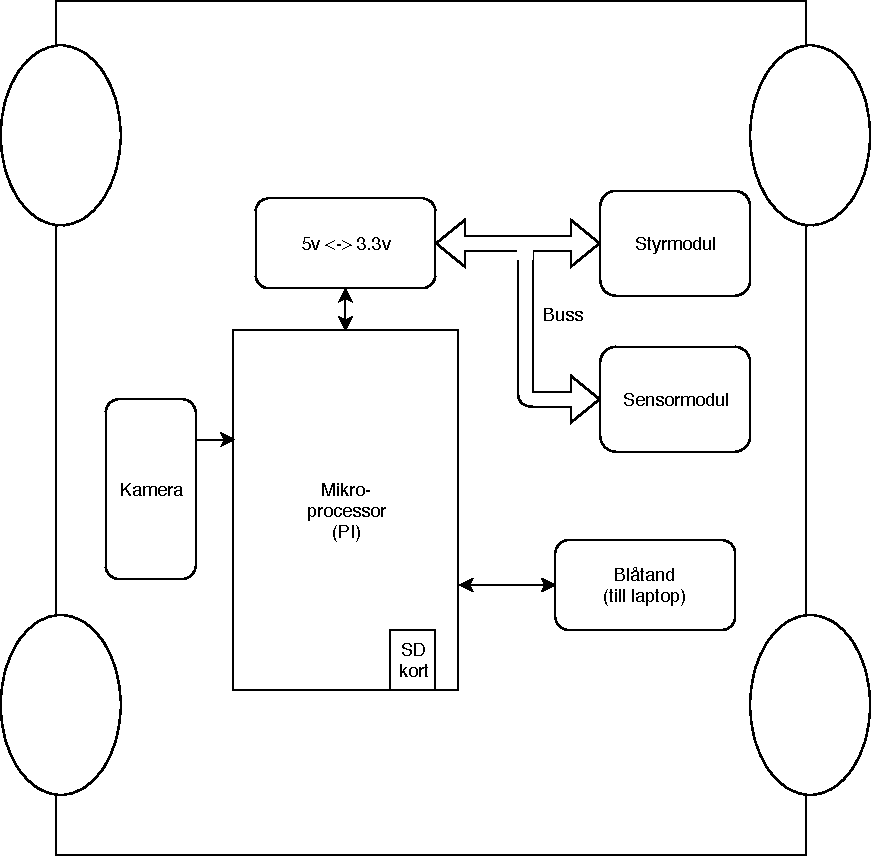
\includegraphics[width=0.6\linewidth]{systemskiss/figures/kommodul.pdf}
    \caption{Övergripande bild över komunikationsmodulen}
    \label{fig:komskiss}
\end{figure}

\noindent
Processorn i modulen kommer vara en Raspberry Pi 3. Den är kraftfull och
utrustad med en rad verktyg som modulen kan ha användning av. Bland annat att
kunna koppla kameran som systemet ska använda för navigering via
bildbehandling. Den har också tillräckligt stort minne som kan användas till
att förvara större programbibliotek och bilder. Processorn har även stöd för
att koppla in trådlösa enheter, vilket gör att den bärbara datorn lätt kan
anslutas. Modulen ska vara kopplad via någon typ av databuss till både styr-
och sensormodulen. För att den kopplingen ska vara möjlig behövs ett filter
eller en nivåskiftare som gör om övriga systemets 5-voltspänningar till
processorns 3.3-voltpinnar.  En enkel skiss av modulen finns i figur
\ref{fig:komskiss}.

\end{document}

